\documentclass[]{article}
\usepackage{graphicx}
\graphicspath{ {graphs/} }
\usepackage{geometry}
\usepackage{gensymb}
\usepackage{booktabs}

%opening
\title{Identification of DC Pixels using Boosted Decision Trees}
\author{Robert Stein}
\begin{document}

\maketitle

\begin{abstract}
A new method of Direct Cherenkov (DC) pixel identification, relying on machine learning, was developed. A set of Cosmic Ray telescope images for training were each simulated twice, both with and without the Extended Air Shower (EAS) background, enabling the DC pixel in every realistic telescope images to be reliably identified using the corresponding background-free image. Using all pixels from these realistic training images, a Boosted Decision Tree (BDT) was trained to identify DC pixels. The BDT performance was tested on a second set of test realistic telescope images, and compared to existing methods of DC pixel identification.  
\end{abstract}

\section{Introduction}
In Cosmic Ray air showers, the primary particle will often emit DC light in the upper atmosphere, before generating an EAS in interaction with the lower atmosphere. In telescope images, this DC light is usually concentrated in a single  \textquoteleft DC pixel'. Identifying this pixel is challenging, because the DC light is much fainter than that from the EAS, which will be recorded in the DC pixel and many of surrounding pixels. As a result, most telescope images will have many bright pixels adjacent to one another, among which one will be the DC pixel. However, if found, the DC pixel can indicate the primary particle energy and charge. 

Currently, the DC pixel is identified after applying a number of cuts first, used a method developed by the HESS collaboration \cite{hess07}. From the subset of events passing these cuts, the variable \[Q_{DC} = \frac{Intensity}{Intensity_{N.N.max}}\] is defined as the ratio of the intensity of a pixel to the largest neighbouring pixel intensity. The DC pixel candidate is simply that with the largest $Q_{DC}$ among those passing the cuts. However, this method is neither reliable nor efficient. An improved method would aim to increase the number of correctly identified events, and enable cuts which better discriminate between correctly and incorrectly identified events.

Using the CORSIKA package, Cosmic Ray events were simulated both with and without an EAS component. The sim\textunderscore telarray package was used to simulate the resultant telescope image, assuming the events were observed by the HESS telescope array. Using the EAS-free image to reliably identify the DC pixel, a Boosted Decision Tree (BDT) was trained on each pixel from a training set of telescope images. The pixel information was provided in the form of individual pixel entries, rather than as discrete sets for images or events.

Thus, once trained, the BDT was applied to every pixel entry in a 'testing' set of simulated telescope images. For each pixel, the BDT assigned a 'Signal Probability', $P_{signal}$, indicating the likelihood of the pixel being the DC pixel. From an entire image, the pixel with the largest $P_{signal}$ was identified as the DC pixel candidate. Repeating the double simulation technique for the test data, the true DC pixels in the test telescope images were reliably identified from EAS-free images. Thus, we can calculate the accuracy of BDT identification for test telescope images.

\section{Image Simulation}
A full simulation of Cosmic Ray air showers was performed using the CORSIKA package \cite{Heck98}, assuming a standard atmospheric profile derived from measurements conducted at the HESS site in Namibia. The simulated particles were $Fe^{56}$, within the Energy Range of $35-135$ TeV and a spectrum $\phi \propto E^{-2.7}$. For each set of simulated event, 4 unique random number seeds were used to generate the shower. An altitude of 1800m was assumed, again corresponding to the HESS site. The simulated zenith angle ranged from $0\degree < \theta < 2 \degree$, while the simulated azimuth angle ranges from $-2\degree < \phi < 2 \degree$. The four smaller HESS-phase-1 telescopes were arranged in a cross along the x/y axis with the larger HESS-phase-2 \textquoteleft CT5' telescope placed at the center. The length of each cross arm was $85m$. The simulated target region of the cores was chosen to be a square centered on CT5, with each 300m-long side bisecting the x/y axis.

In order to identify the DC pixel, a \textquoteleft DC Simulation' was initially run with an energy cut of 10 PeV on all muons and electrons. The consequence of this was to ensure that only the Cherenkov Light from the primary particle, as well as its fragments, was simulated. A second identical \textquoteleft Full Simulation' was run including the same random seeds, but without the energy cut on muons and electrons. This gave a complete air shower including the DC light, representative of those imaged in telescope arrays. Comparisons of the Full and DC simulations enabled us to identify background light in the Full shower.

Using the sim\textunderscore telarray package \cite{Bernlohr08}, the expected hardware response to an air shower can be simulated. Again, the built-in response of the HESS telescope was selected for simulation. The program accounts for atmospheric transmission and density, mirror positions, sizes and reflectivities, camera shadowing and triggering, quantum efficiency and pulse responses. Due to the comprehensive and detailed nature of these hardware simulations, the resultant images can be considered representative of true camera images. For the Full Simulation, the night sky background was also simulated by sim\textunderscore telarray.

The HESS telescope has both a high gain Channel 0 and a low gain Channel 1. The location of each pixel (dependent on camera size), alongside the Sim\textunderscore telarray simulated value of SOMETHING? in each value was extracted. The pedestal and gain for each channel was also recorded, and from this, Intensity can be found.

\[ Intensity = (Count - Pedestal)\times Gain \]

In the case of many iron core events, Channel 0 will reach its maximum value and become saturated. Thus Channel 0 ceases to be useful for discriminating between high energy DC and non-DC pixels, so was not used in this analysis. Instead, only the Channel 1 was used in later analysis. Thus the Channel 1 Intensity will simply be referred to throughout this analysis as $Intensity$. 

In addition to the $Intensity$ of each pixel, the Sim\textunderscore telarray derives various Hillas whole-image parameters, which the script also extracted. These include the image width and length measured in degrees, from which the aspect ratio $A.R = \frac{width}{length}$ was calculated. Further the reconstructed shower direction and the shower center of gravity were calculated as positions in azimuth and zenith. Additionally the calculated energy and distance to core $r_{core}$ were recorded.

An entry was constructed for every pixel, containing its count and position. The variables $ \Delta_{C.o.G}$, $\Delta_{Direction}$ and $\Delta_{Line}$ were defined as the distance from the pixel to the shower center of gravity, shower direction, and the line joining those two points. Furthermore, the nearest neigbouring pixel IDs were calculated for every pixel position, enabling the count in each neighbouring pixel to be found. From this, two further pixel variables were defined. The largest neighbouring intensity $Intensity_{N.N.max}$ was found, and the ratio $ Q_{DC} = \frac{Intensity}{Intensity_{N.N.max}} $ was derived. In addition the Nearest Neighbour Mean Count was recorded. These variables were recorded in every pixel entry, and together the pixel entries formed a complete dataset for each camera image.

\subsection{Classic DC Identification}
The original method used by the HESS collaboration \cite{hess07} was initially replicated, for which a number of cuts were applied to each image dataset.

\begin{table}[h!]
  \centering
  \caption{Cuts applied to image pixel sets}
  \label{tab:table1}
  \begin{tabular}{ccc}
    \toprule
    Variable & Cut\\
    \midrule
     $r_{core}$ & \textgreater 0.4 \\
     $Q_{DC}$ & \textgreater 1.3 \\
     $ \Delta_{C.o.G}$ & \textgreater 0.17 \\
     $ \Delta_{C.o.G}$ & \textless 0.91 \\
     $\Delta_{Direction}$ & \textless 0.45 \\
     $\Delta_{Line}$ & \textless 0.23 \\
     Aspect Ratio & \textless 0.75 \\
    \bottomrule
  \end{tabular}
\end{table}

From the subset of pixels satisfying these conditions, the remaining pixel with the largest $Q_{DC}$ was selected as the DC pixel. The result was compared with the true DC pixel, identified from the hadron-only image, to test the accuracy of this cut. Out of 400 events, it was fount that only 55\% of these events contained a clear DC signal, as defined by requiring the DC pixel to have $Intensity_{DC} > 150$ in the hadron-only image. SOMETHING! Of this subset of 'DC events', 17\% events passed all of the required cuts. The $Q_{DC}$ was found to be 100\% accurate in identifying the DC pixel in those passing events, as shown in \ref{fig:cutdistribution}.

\begin{figure}
\begin{center}
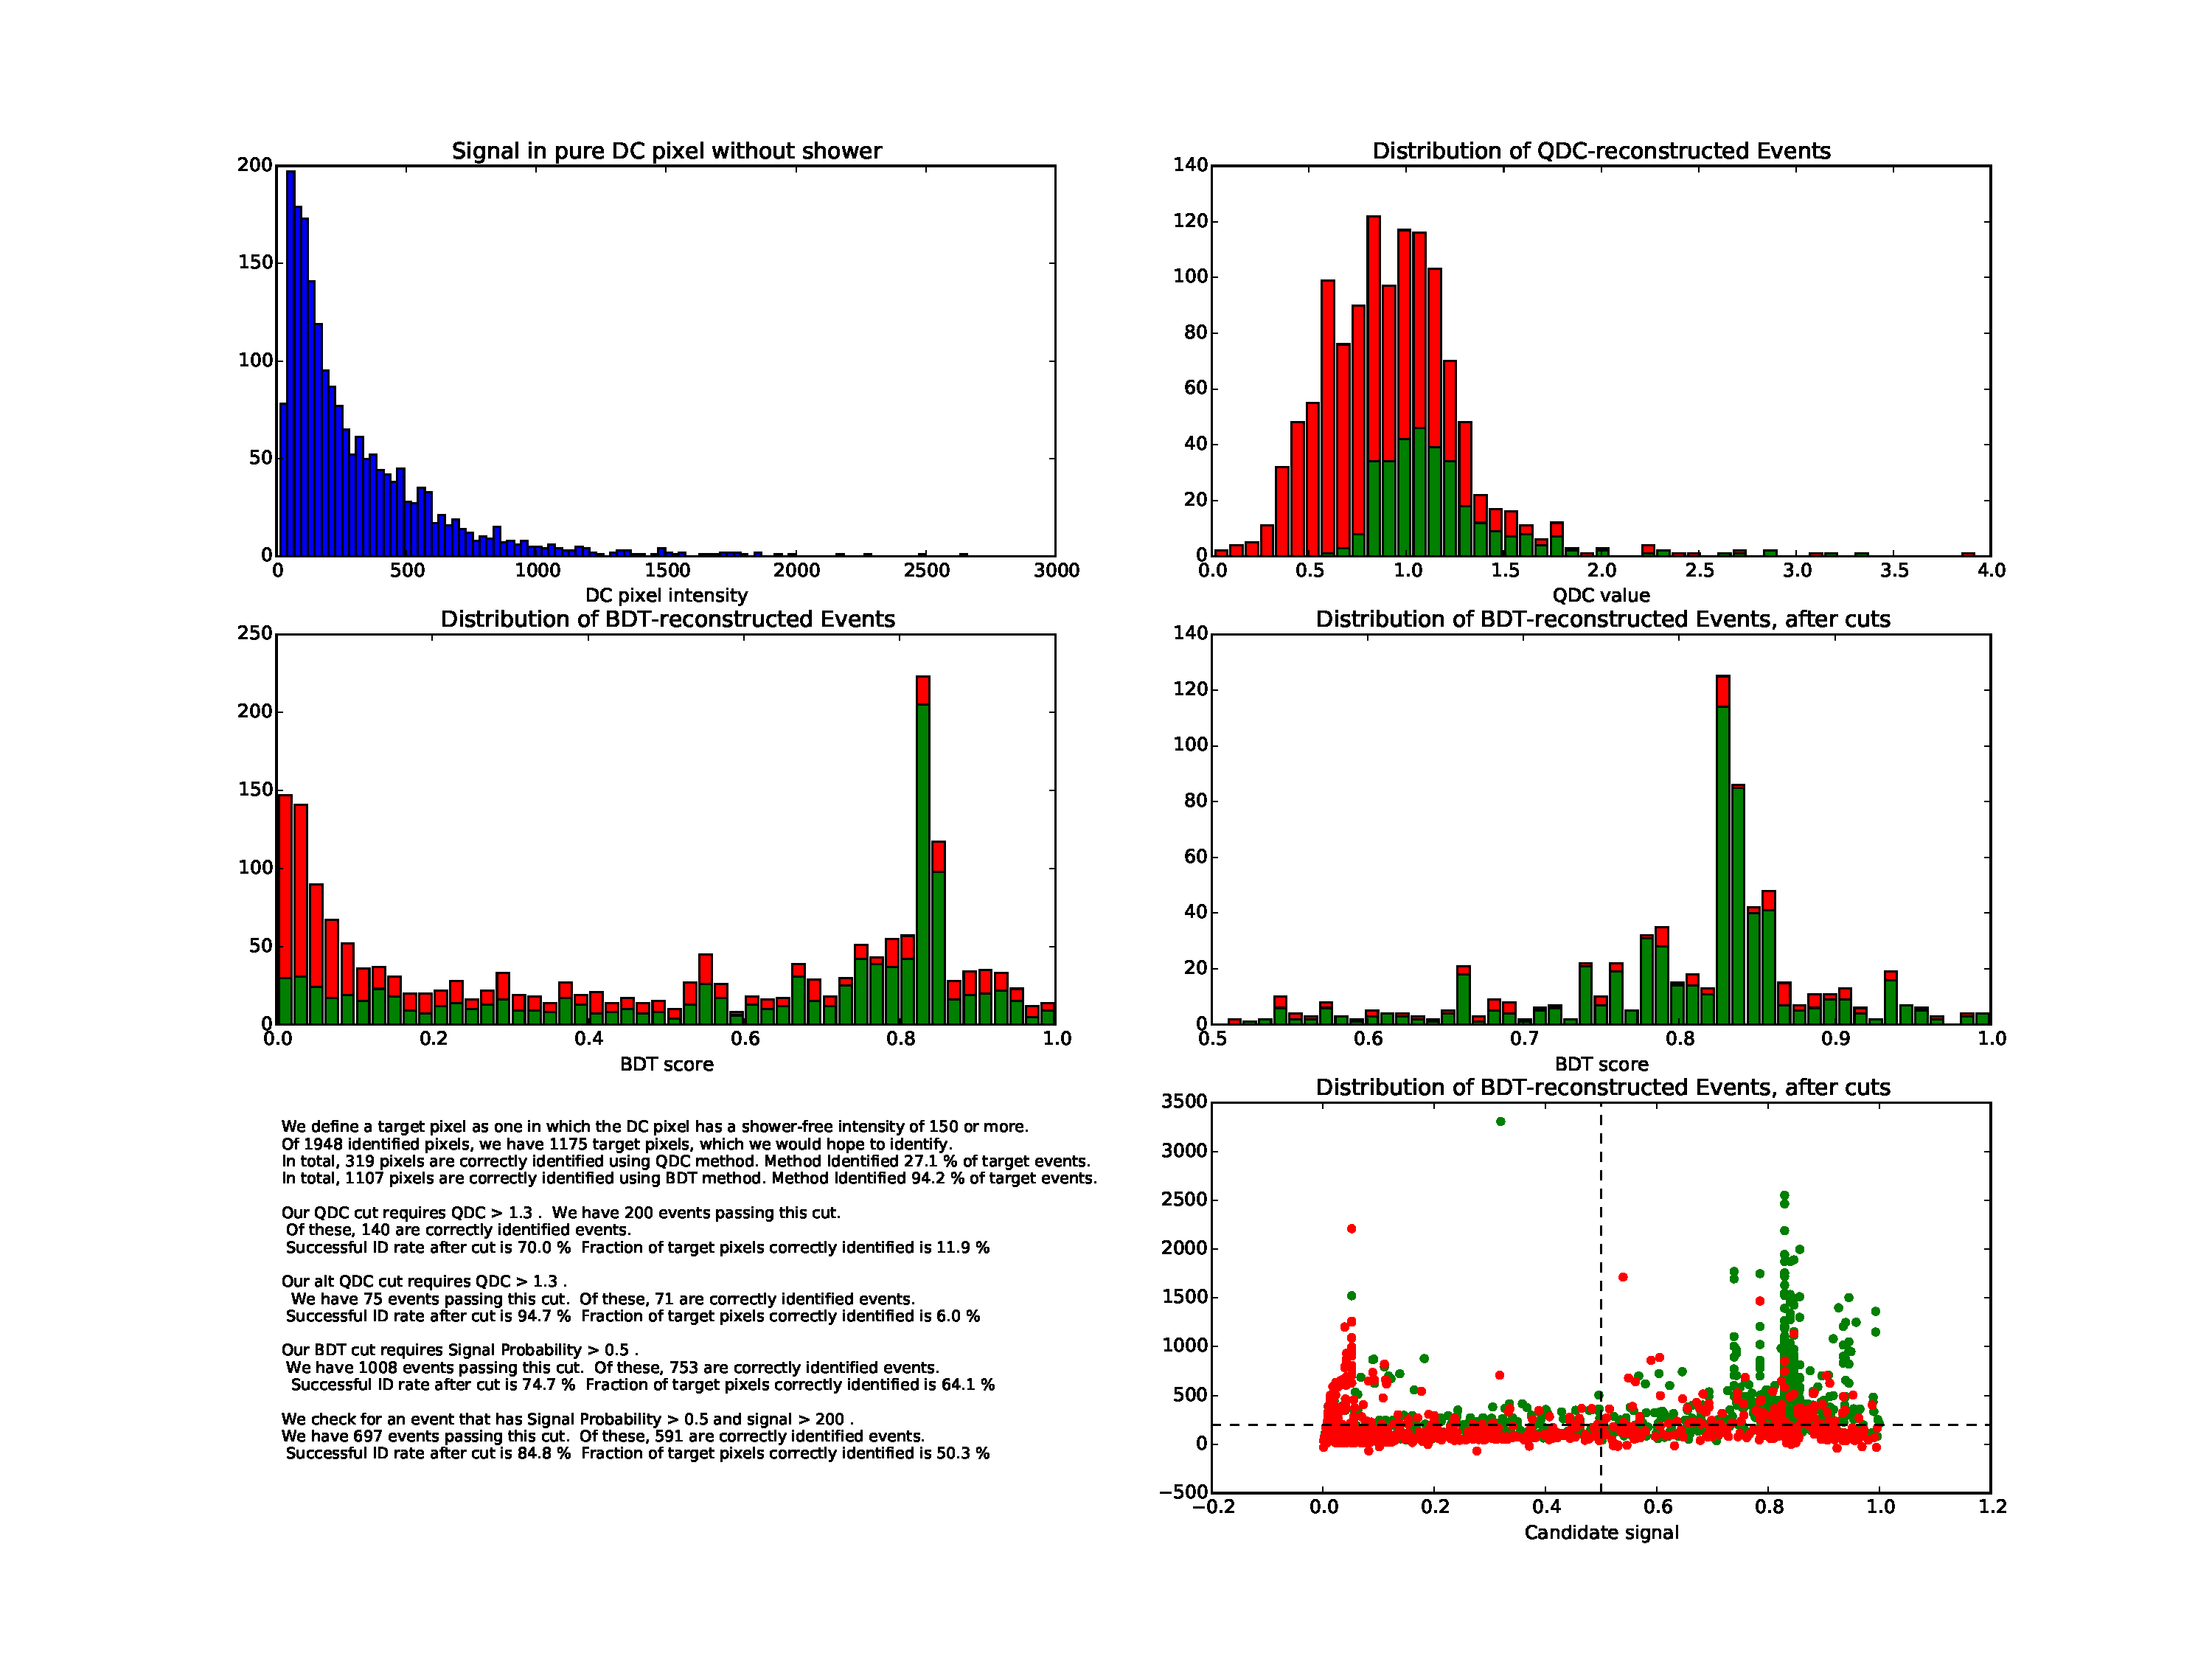
\includegraphics[width=\textwidth]{cutdistributionhess1None}
\caption{The DC signal in the shower-free pixel is shown in the top left, with a broad gaussian distribution with the tail of the night-sky background extending up to appproximately 5000. Events below this are unlikely to be identified correctly because the DEC light is too faint. In the top right- the distribution of the dataset is shown, once all the non-$Q_{DC}$ cuts have been applied. In the bottom left, the BDT score distribution is shown before any cuts. On the bottom right, we see the same distribution after both signal and BDT score cuts are applied. All green events are ones in which the DC pixel has been correctly identified, while red events are ones that have been incorrectly identified.}
\label{fig:cutdistribution}
\end{center}
\end{figure} 

\subsection{Boosted Decision Tree DC Identification}  As an alternative to use of $Q_{DC}$, a new method of DC pixel identification was developed as part of this analysis by using a BDT trained with the Scikit Learn Python package. A set of 2000 simulated events was selected, and randomly split through use of the python random.random() function into two subsets for training and testing. The variable $DC_{Count} = Count-Mean_{N.N}$ was defined as an approximate \textquoteleft DC signal', if the pixel were to be selected as the DC candidate. For every pixel in the 2000 simulated events HESS 1 images, an entry was formed of $Q_{DC}$, $ \Delta_{C.o.G}$, $\Delta_{Direction}$, $\Delta_{Line}$, Channel1, Channel0, $DC_{Count}$ and $Mean_{N.N}$. A score of 0 was assigned to every pixel to indicate background, with the exception of those that were identified as the DC pixel through the Shower-Free simulation. If the DC count in the shower-free simulation was larger than 300, the pixel was included with a score of 1, identifying it as a signal pixel. Pure DC pixels below the threshold cut of 300 were deemed to be too faint to reconstruct, so these entries were omitted from the training set.

Having created a dataset, the BDT was then trained with a maximum depth of 5, and 100 trees generated. It was found that the BDT was 100 \% accurate for the entire training dataset, with a breakdown of 100 \% for the training background and 99 \% accurate with the training signal. When the trained BDT was applied to the testing pixels, it was found to be 99.99 \%  accurate for the entire training dataset, with a breakdown of 100 \% for the testing background and 99 \% accurate with the testing signal. This indicates that the BDT was not significantly overtrained, which would otherwise be manifested by a large divergence in accuracy between testing and training data.

\subsection{Composite Event Selection}
Having trained the BDT successfully, it was then applied to the same dataset as for the classic QDC identification. In each camera image, the event with the largest BDT score was deemed to be \textquoteleft most signal-like', and thus selected as the DC pixel candidate. A cut was applied, requiring $Probability_{signal} > 0.5$ for the DC candidate to be accepted. 

With this cut applied, out of 1200 events, 46\% events passed all of the required cuts. The BDT was found to be 85 \% accurate in identifying the DC pixel in those passing events.

In \ref{fig:cutdistribution}, a plot of true vs. reconstructed DC count is shown, obtained by comparing the BDT selected pixel to the hadron-only DC pixel. The black line indicates the optimal 1:1 ratio that we are aiming for. It is seen that there the vast majority of misidentified events have a small $candidate_{DC count}$, forming a red line in the region $candidate_{DC count} \approx 0$. To remove these misidentified events, we can apply a second cut requiring $candidate_{DC count} > 300$.

Application of this combined cut greatly increases the successful identification rate. Of the 2000 events, 84\% of events passed all of the required cuts. The BDT was found to be 90 \% accurate in identifying the DC pixel in those passing events. This represents a very significant improvement in DC pixel identification over the previous QDC method, and corresponds to a fivefold increase in the number of HESS data events that can be studied using the LPD method. Use of this BDT method is thus assumed throughout the rest of this analysis.

\subsection{Error in calculated $Count_{DC}$}
Having successfully identified the DC pixel in many events, we can calculate the difference between the derived $candidate_{DC count}$ and the hadron-only $True_{DC}$ to determine the error we will find for the LPD. Binning the difference $\Delta = candidate_{DC count} - True_{DC count}$ as shown in FIG, we find that the mean difference is 65 and the median difference is -75. We thus see that the distribution is not significantly skewed. However, the Standard deviation is approximately 600 when measured both by half of the difference from the 16th to 84th centile, and by 68th centile of an absolute difference. This again suggests that, although skewed, the fraction error in intensity is rather large. However, the fractional error found purely on the basis of QDC calculations is EQUALLY LARGE??LARGER?.

\begin{figure}
\begin{center}
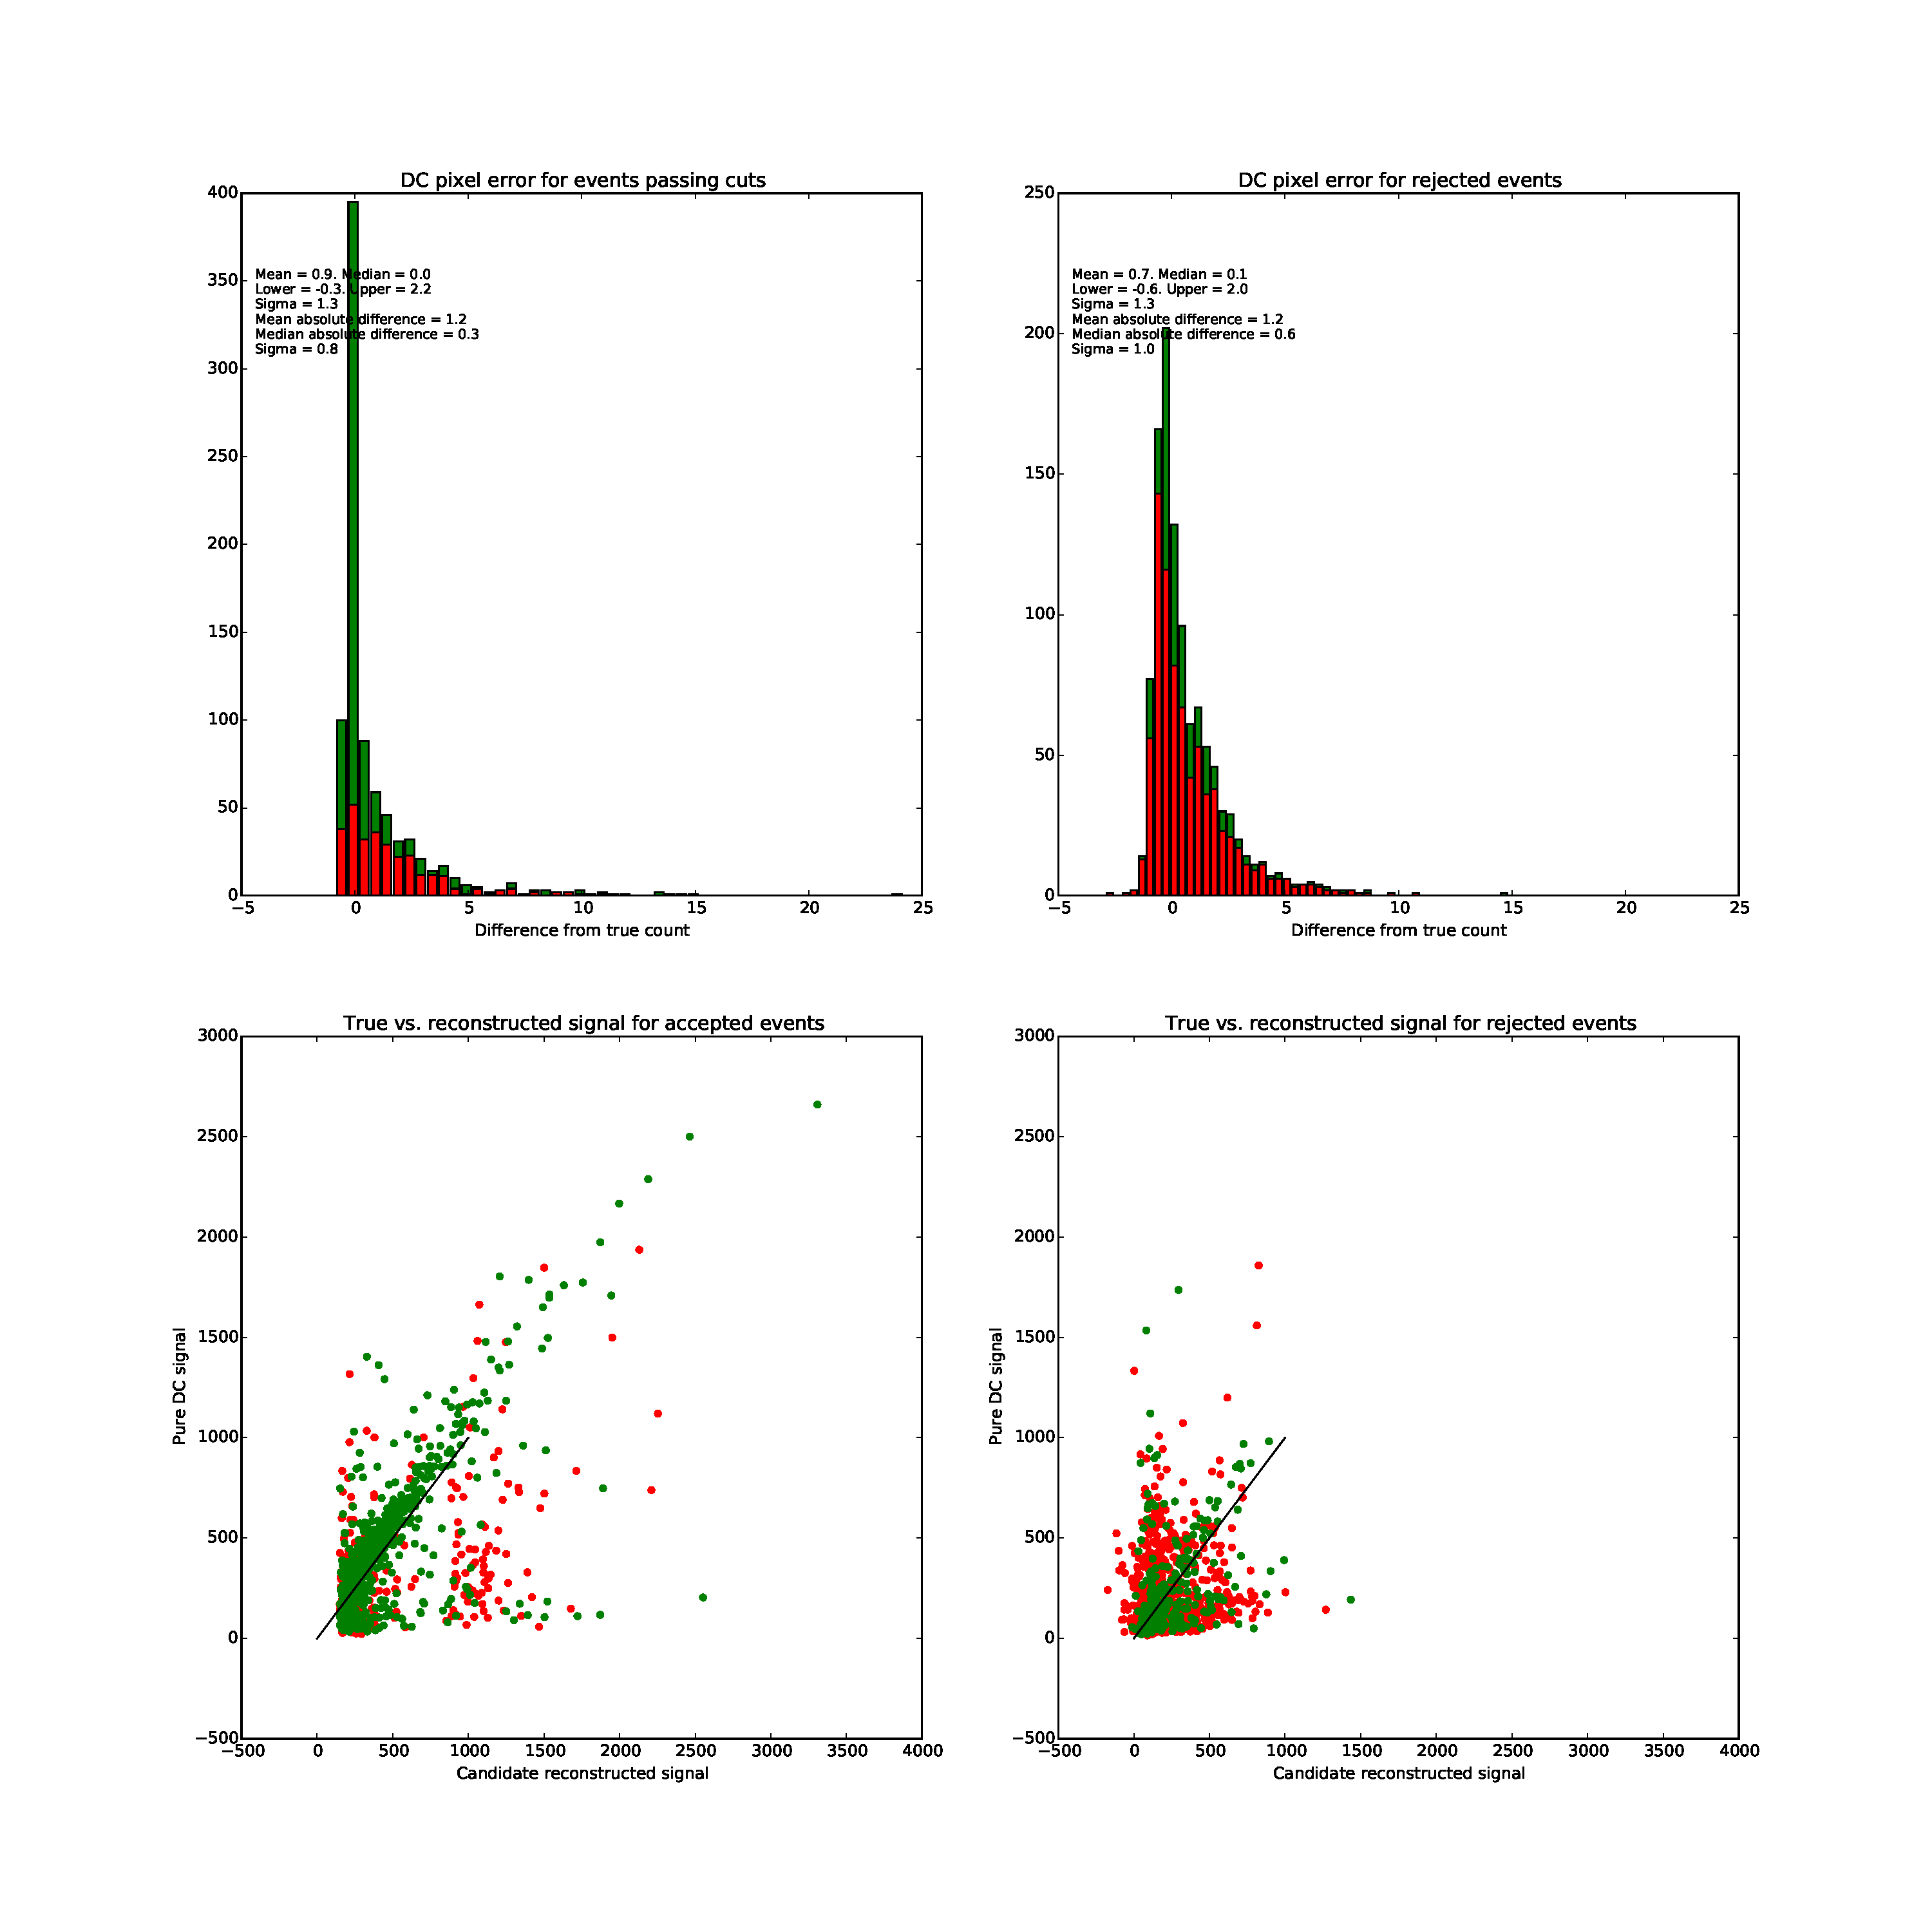
\includegraphics[width=\textwidth]{DCcounterrorhess1}
\caption{The difference between true and reconstructed DC signal for events passing the cuts is shown in the top left. In the top right the same is shown for events which were rejected. The true DC signals for events which passed the cuts is plotted against the reconstructed signals in the lower left, and for rejected events in the lower right. As in \ref{fig:cutdistribution}, in all plots a green event is one in which the DC pixel has been correctly identified, while a red event is one that has been incorrectly identified.}
\label{fig:dcdiff}
\end{center}
\end{figure}

\bibliographystyle{plain}
\bibliography{report}

\end{document}
